\documentclass[1p]{elsarticle_modified}
%\bibliographystyle{elsarticle-num}

%\usepackage[colorlinks]{hyperref}
%\usepackage{abbrmath_seonhwa} %\Abb, \Ascr, \Acal ,\Abf, \Afrak
\usepackage{amsfonts}
\usepackage{amssymb}
\usepackage{amsmath}
\usepackage{amsthm}
\usepackage{scalefnt}
\usepackage{amsbsy}
\usepackage{kotex}
\usepackage{caption}
\usepackage{subfig}
\usepackage{color}
\usepackage{graphicx}
\usepackage{xcolor} %% white, black, red, green, blue, cyan, magenta, yellow
\usepackage{float}
\usepackage{setspace}
\usepackage{hyperref}

\usepackage{tikz}
\usetikzlibrary{arrows}

\usepackage{multirow}
\usepackage{array} % fixed length table
\usepackage{hhline}

%%%%%%%%%%%%%%%%%%%%%
\makeatletter
\renewcommand*\env@matrix[1][\arraystretch]{%
	\edef\arraystretch{#1}%
	\hskip -\arraycolsep
	\let\@ifnextchar\new@ifnextchar
	\array{*\c@MaxMatrixCols c}}
\makeatother %https://tex.stackexchange.com/questions/14071/how-can-i-increase-the-line-spacing-in-a-matrix
%%%%%%%%%%%%%%%

\usepackage[normalem]{ulem}

\newcommand{\msout}[1]{\ifmmode\text{\sout{\ensuremath{#1}}}\else\sout{#1}\fi}
%SOURCE: \msout is \stkout macro in https://tex.stackexchange.com/questions/20609/strikeout-in-math-mode

\newcommand{\cancel}[1]{
	\ifmmode
	{\color{red}\msout{#1}}
	\else
	{\color{red}\sout{#1}}
	\fi
}

\newcommand{\add}[1]{
	{\color{blue}\uwave{#1}}
}

\newcommand{\replace}[2]{
	\ifmmode
	{\color{red}\msout{#1}}{\color{blue}\uwave{#2}}
	\else
	{\color{red}\sout{#1}}{\color{blue}\uwave{#2}}
	\fi
}

\newcommand{\Sol}{\mathcal{S}} %segment
\newcommand{\D}{D} %diagram
\newcommand{\A}{\mathcal{A}} %arc


%%%%%%%%%%%%%%%%%%%%%%%%%%%%%5 test

\def\sl{\operatorname{\textup{SL}}(2,\Cbb)}
\def\psl{\operatorname{\textup{PSL}}(2,\Cbb)}
\def\quan{\mkern 1mu \triangleright \mkern 1mu}

\theoremstyle{definition}
\newtheorem{thm}{Theorem}[section]
\newtheorem{prop}[thm]{Proposition}
\newtheorem{lem}[thm]{Lemma}
\newtheorem{ques}[thm]{Question}
\newtheorem{cor}[thm]{Corollary}
\newtheorem{defn}[thm]{Definition}
\newtheorem{exam}[thm]{Example}
\newtheorem{rmk}[thm]{Remark}
\newtheorem{alg}[thm]{Algorithm}

\newcommand{\I}{\sqrt{-1}}
\begin{document}

%\begin{frontmatter}
%
%\title{Boundary parabolic representations of knots up to 8 crossings}
%
%%% Group authors per affiliation:
%\author{Yunhi Cho} 
%\address{Department of Mathematics, University of Seoul, Seoul, Korea}
%\ead{yhcho@uos.ac.kr}
%
%
%\author{Seonhwa Kim} %\fnref{s_kim}}
%\address{Center for Geometry and Physics, Institute for Basic Science, Pohang, 37673, Korea}
%\ead{ryeona17@ibs.re.kr}
%
%\author{Hyuk Kim}
%\address{Department of Mathematical Sciences, Seoul National University, Seoul 08826, Korea}
%\ead{hyukkim@snu.ac.kr}
%
%\author{Seokbeom Yoon}
%\address{Department of Mathematical Sciences, Seoul National University, Seoul, 08826,  Korea}
%\ead{sbyoon15@snu.ac.kr}
%
%\begin{abstract}
%We find all boundary parabolic representation of knots up to 8 crossings.
%
%\end{abstract}
%\begin{keyword}
%    \MSC[2010] 57M25 
%\end{keyword}
%
%\end{frontmatter}

%\linenumbers
%\tableofcontents
%
\newcommand\colored[1]{\textcolor{white}{\rule[-0.35ex]{0.8em}{1.4ex}}\kern-0.8em\color{red} #1}%
%\newcommand\colored[1]{\textcolor{white}{ #1}\kern-2.17ex	\textcolor{white}{ #1}\kern-1.81ex	\textcolor{white}{ #1}\kern-2.15ex\color{red}#1	}

{\Large $\underline{11a_{52}~(K11a_{52})}$}

\setlength{\tabcolsep}{10pt}
\renewcommand{\arraystretch}{1.6}
\vspace{1cm}\begin{tabular}{m{100pt}>{\centering\arraybackslash}m{274pt}}
\multirow{5}{120pt}{
	\centering
	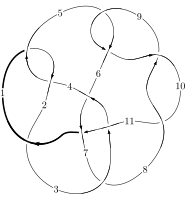
\includegraphics[width=112pt]{../../../GIT/diagram.site/Diagrams/png/301_11a_52.png}\\
\ \ \ A knot diagram\footnotemark}&
\allowdisplaybreaks
\textbf{Linearized knot diagam} \\
\cline{2-2}
 &
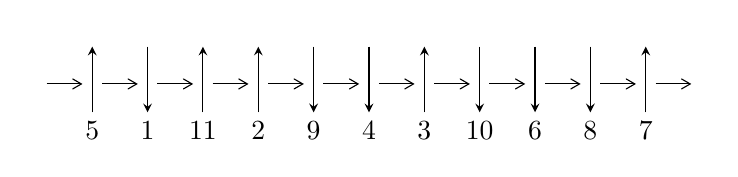
\begin{tikzpicture}[x=20pt, y=17pt]
	% nodes
	\node (C0) at (0, 0) {};
	\node (C1) at (1, 0) {};
	\node (C1U) at (1, +1) {};
	\node (C1D) at (1, -1) {5};

	\node (C2) at (2, 0) {};
	\node (C2U) at (2, +1) {};
	\node (C2D) at (2, -1) {1};

	\node (C3) at (3, 0) {};
	\node (C3U) at (3, +1) {};
	\node (C3D) at (3, -1) {11};

	\node (C4) at (4, 0) {};
	\node (C4U) at (4, +1) {};
	\node (C4D) at (4, -1) {2};

	\node (C5) at (5, 0) {};
	\node (C5U) at (5, +1) {};
	\node (C5D) at (5, -1) {9};

	\node (C6) at (6, 0) {};
	\node (C6U) at (6, +1) {};
	\node (C6D) at (6, -1) {4};

	\node (C7) at (7, 0) {};
	\node (C7U) at (7, +1) {};
	\node (C7D) at (7, -1) {3};

	\node (C8) at (8, 0) {};
	\node (C8U) at (8, +1) {};
	\node (C8D) at (8, -1) {10};

	\node (C9) at (9, 0) {};
	\node (C9U) at (9, +1) {};
	\node (C9D) at (9, -1) {6};

	\node (C10) at (10, 0) {};
	\node (C10U) at (10, +1) {};
	\node (C10D) at (10, -1) {8};

	\node (C11) at (11, 0) {};
	\node (C11U) at (11, +1) {};
	\node (C11D) at (11, -1) {7};
	\node (C12) at (12, 0) {};

	% arrows
	\draw[->,>={angle 60}]
	(C0) edge (C1) (C1) edge (C2) (C2) edge (C3) (C3) edge (C4) (C4) edge (C5) (C5) edge (C6) (C6) edge (C7) (C7) edge (C8) (C8) edge (C9) (C9) edge (C10) (C10) edge (C11) (C11) edge (C12) ;	\draw[->,>=stealth]
	(C1D) edge (C1U) (C2U) edge (C2D) (C3D) edge (C3U) (C4D) edge (C4U) (C5U) edge (C5D) (C6U) edge (C6D) (C7D) edge (C7U) (C8U) edge (C8D) (C9U) edge (C9D) (C10U) edge (C10D) (C11D) edge (C11U) ;
	\end{tikzpicture} \\
\hhline{~~} \\& 
\textbf{Solving Sequence} \\ \cline{2-2} 
 &
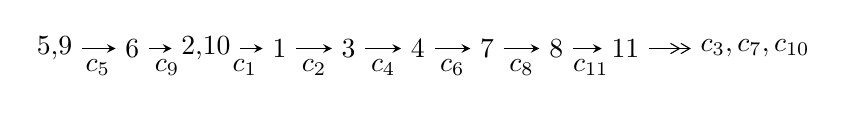
\begin{tikzpicture}[x=25pt, y=7pt]
	% node
	\node (A0) at (-1/8, 0) {5,9};
	\node (A1) at (1, 0) {6};
	\node (A2) at (33/16, 0) {2,10};
	\node (A3) at (25/8, 0) {1};
	\node (A4) at (33/8, 0) {3};
	\node (A5) at (41/8, 0) {4};
	\node (A6) at (49/8, 0) {7};
	\node (A7) at (57/8, 0) {8};
	\node (A8) at (65/8, 0) {11};
	\node (C1) at (1/2, -1) {$c_{5}$};
	\node (C2) at (3/2, -1) {$c_{9}$};
	\node (C3) at (21/8, -1) {$c_{1}$};
	\node (C4) at (29/8, -1) {$c_{2}$};
	\node (C5) at (37/8, -1) {$c_{4}$};
	\node (C6) at (45/8, -1) {$c_{6}$};
	\node (C7) at (53/8, -1) {$c_{8}$};
	\node (C8) at (61/8, -1) {$c_{11}$};
	\node (A9) at (10, 0) {$c_{3},c_{7},c_{10}$};

	% edge
	\draw[->,>=stealth]	
	(A0) edge (A1) (A1) edge (A2) (A2) edge (A3) (A3) edge (A4) (A4) edge (A5) (A5) edge (A6) (A6) edge (A7) (A7) edge (A8) ;
	\draw[->>,>={angle 60}]	
	(A8) edge (A9);
\end{tikzpicture} \\ 

\end{tabular} \\

\footnotetext{
The image of knot diagram is generated by the software ``\textbf{Draw programme}" developed by Andrew Bartholomew(\url{http://www.layer8.co.uk/maths/draw/index.htm\#Running-draw}), where we modified some parts for our purpose(\url{https://github.com/CATsTAILs/LinksPainter}).
}\phantom \\ \newline 
\centering \textbf{Ideals for irreducible components\footnotemark of $X_{\text{par}}$} 
 
\begin{align*}
I^u_{1}&=\langle 
-2.36254\times10^{45} u^{69}+4.82278\times10^{45} u^{68}+\cdots+1.20308\times10^{45} b+1.54557\times10^{45},\\
\phantom{I^u_{1}}&\phantom{= \langle  }-8.19355\times10^{45} u^{69}+1.66575\times10^{46} u^{68}+\cdots+1.20308\times10^{45} a+9.02950\times10^{45},\;u^{70}-3 u^{69}+\cdots+2 u+1\rangle \\
I^u_{2}&=\langle 
3 b- a-1,\;a^2- a+7,\;u-1\rangle \\
\\
\end{align*}
\raggedright * 2 irreducible components of $\dim_{\mathbb{C}}=0$, with total 72 representations.\\
\footnotetext{All coefficients of polynomials are rational numbers. But the coefficients are sometimes approximated in decimal forms when there is not enough margin.}
\newpage
\renewcommand{\arraystretch}{1}
\centering \section*{I. $I^u_{1}= \langle -2.36\times10^{45} u^{69}+4.82\times10^{45} u^{68}+\cdots+1.20\times10^{45} b+1.55\times10^{45},\;-8.19\times10^{45} u^{69}+1.67\times10^{46} u^{68}+\cdots+1.20\times10^{45} a+9.03\times10^{45},\;u^{70}-3 u^{69}+\cdots+2 u+1 \rangle$}
\flushleft \textbf{(i) Arc colorings}\\
\begin{tabular}{m{7pt} m{180pt} m{7pt} m{180pt} }
\flushright $a_{5}=$&$\begin{pmatrix}1\\0\end{pmatrix}$ \\
\flushright $a_{9}=$&$\begin{pmatrix}0\\u\end{pmatrix}$ \\
\flushright $a_{6}=$&$\begin{pmatrix}1\\u^2\end{pmatrix}$ \\
\flushright $a_{2}=$&$\begin{pmatrix}6.81046 u^{69}-13.8457 u^{68}+\cdots-19.7949 u-7.50529\\1.96374 u^{69}-4.00868 u^{68}+\cdots-1.36136 u-1.28468\end{pmatrix}$ \\
\flushright $a_{10}=$&$\begin{pmatrix}- u\\- u^3+u\end{pmatrix}$ \\
\flushright $a_{1}=$&$\begin{pmatrix}4.84672 u^{69}-9.83700 u^{68}+\cdots-18.4335 u-6.22062\\1.96374 u^{69}-4.00868 u^{68}+\cdots-1.36136 u-1.28468\end{pmatrix}$ \\
\flushright $a_{3}=$&$\begin{pmatrix}-22.4801 u^{69}+51.8492 u^{68}+\cdots+114.630 u+32.1980\\0.955391 u^{69}-1.83843 u^{68}+\cdots+1.87417 u+0.890916\end{pmatrix}$ \\
\flushright $a_{4}=$&$\begin{pmatrix}24.1027 u^{69}-55.6549 u^{68}+\cdots-122.558 u-34.6348\\-1.26457 u^{69}+2.55163 u^{68}+\cdots-0.684959 u-0.355838\end{pmatrix}$ \\
\flushright $a_{7}=$&$\begin{pmatrix}15.0245 u^{69}-34.6120 u^{68}+\cdots-70.5010 u-21.5396\\-2.29156 u^{69}+4.76568 u^{68}+\cdots+9.69809 u+2.33641\end{pmatrix}$ \\
\flushright $a_{8}=$&$\begin{pmatrix}u^3\\u^5- u^3+u\end{pmatrix}$ \\
\flushright $a_{11}=$&$\begin{pmatrix}- u^5- u\\- u^7+u^5-2 u^3+u\end{pmatrix}$\\ \flushright $a_{11}=$&$\begin{pmatrix}- u^5- u\\- u^7+u^5-2 u^3+u\end{pmatrix}$\\&\end{tabular}
\flushleft \textbf{(ii) Obstruction class $= -1$}\\~\\
\flushleft \textbf{(iii) Cusp Shapes $= -136.960 u^{69}+306.752 u^{68}+\cdots+605.662 u+186.864$}\\~\\
\newpage\renewcommand{\arraystretch}{1}
\flushleft \textbf{(iv) u-Polynomials at the component}\newline \\
\begin{tabular}{m{50pt}|m{274pt}}
Crossings & \hspace{64pt}u-Polynomials at each crossing \\
\hline $$\begin{aligned}c_{1},c_{4}\end{aligned}$$&$\begin{aligned}
&u^{70}+2 u^{69}+\cdots+7 u+1
\end{aligned}$\\
\hline $$\begin{aligned}c_{2}\end{aligned}$$&$\begin{aligned}
&u^{70}+26 u^{69}+\cdots-61 u+1
\end{aligned}$\\
\hline $$\begin{aligned}c_{3}\end{aligned}$$&$\begin{aligned}
&u^{70}+7 u^{69}+\cdots-4 u+4
\end{aligned}$\\
\hline $$\begin{aligned}c_{5},c_{9}\end{aligned}$$&$\begin{aligned}
&u^{70}+3 u^{69}+\cdots-2 u+1
\end{aligned}$\\
\hline $$\begin{aligned}c_{6}\end{aligned}$$&$\begin{aligned}
&u^{70}-4 u^{69}+\cdots-14859 u+4643
\end{aligned}$\\
\hline $$\begin{aligned}c_{7}\end{aligned}$$&$\begin{aligned}
&u^{70}-2 u^{69}+\cdots+3989 u+641
\end{aligned}$\\
\hline $$\begin{aligned}c_{8},c_{10}\end{aligned}$$&$\begin{aligned}
&u^{70}+21 u^{69}+\cdots+8 u+1
\end{aligned}$\\
\hline $$\begin{aligned}c_{11}\end{aligned}$$&$\begin{aligned}
&u^{70}+7 u^{69}+\cdots-4 u^2+1
\end{aligned}$\\
\hline
\end{tabular}\\~\\
\newpage\renewcommand{\arraystretch}{1}
\flushleft \textbf{(v) Riley Polynomials at the component}\newline \\
\begin{tabular}{m{50pt}|m{274pt}}
Crossings & \hspace{64pt}Riley Polynomials at each crossing \\
\hline $$\begin{aligned}c_{1},c_{4}\end{aligned}$$&$\begin{aligned}
&y^{70}+26 y^{69}+\cdots-61 y+1
\end{aligned}$\\
\hline $$\begin{aligned}c_{2}\end{aligned}$$&$\begin{aligned}
&y^{70}+38 y^{69}+\cdots-1741 y+1
\end{aligned}$\\
\hline $$\begin{aligned}c_{3}\end{aligned}$$&$\begin{aligned}
&y^{70}-15 y^{69}+\cdots-328 y+16
\end{aligned}$\\
\hline $$\begin{aligned}c_{5},c_{9}\end{aligned}$$&$\begin{aligned}
&y^{70}-21 y^{69}+\cdots-8 y+1
\end{aligned}$\\
\hline $$\begin{aligned}c_{6}\end{aligned}$$&$\begin{aligned}
&y^{70}-46 y^{69}+\cdots+512636971 y+21557449
\end{aligned}$\\
\hline $$\begin{aligned}c_{7}\end{aligned}$$&$\begin{aligned}
&y^{70}-90 y^{69}+\cdots-12237909 y+410881
\end{aligned}$\\
\hline $$\begin{aligned}c_{8},c_{10}\end{aligned}$$&$\begin{aligned}
&y^{70}+59 y^{69}+\cdots+128 y+1
\end{aligned}$\\
\hline $$\begin{aligned}c_{11}\end{aligned}$$&$\begin{aligned}
&y^{70}-9 y^{69}+\cdots-8 y+1
\end{aligned}$\\
\hline
\end{tabular}\\~\\
\newpage\flushleft \textbf{(vi) Complex Volumes and Cusp Shapes}
$$\begin{array}{c|c|c}  
\text{Solutions to }I^u_{1}& \I (\text{vol} + \sqrt{-1}CS) & \text{Cusp shape}\\
 \hline 
\begin{aligned}
u &= -0.995386 + 0.165662 I \\
a &= \phantom{-}0.18980 - 2.80256 I \\
b &= \phantom{-}0.036237 - 1.176330 I\end{aligned}
 & -5.59225 + 3.69663 I & \phantom{-0.000000 } 0 \\ \hline\begin{aligned}
u &= -0.995386 - 0.165662 I \\
a &= \phantom{-}0.18980 + 2.80256 I \\
b &= \phantom{-}0.036237 + 1.176330 I\end{aligned}
 & -5.59225 - 3.69663 I & \phantom{-0.000000 } 0 \\ \hline\begin{aligned}
u &= -0.828278 + 0.688700 I \\
a &= -1.33032 + 1.83011 I \\
b &= -0.248336 + 0.844356 I\end{aligned}
 & \phantom{-}1.83973 + 0.97289 I & \phantom{-0.000000 } 0 \\ \hline\begin{aligned}
u &= -0.828278 - 0.688700 I \\
a &= -1.33032 - 1.83011 I \\
b &= -0.248336 - 0.844356 I\end{aligned}
 & \phantom{-}1.83973 - 0.97289 I & \phantom{-0.000000 } 0 \\ \hline\begin{aligned}
u &= \phantom{-}0.996317 + 0.448702 I \\
a &= -1.53721 - 1.79701 I \\
b &= \phantom{-}0.225350 - 0.984742 I\end{aligned}
 & -3.99310 - 2.18696 I & \phantom{-0.000000 } 0 \\ \hline\begin{aligned}
u &= \phantom{-}0.996317 - 0.448702 I \\
a &= -1.53721 + 1.79701 I \\
b &= \phantom{-}0.225350 + 0.984742 I\end{aligned}
 & -3.99310 + 2.18696 I & \phantom{-0.000000 } 0 \\ \hline\begin{aligned}
u &= \phantom{-}0.770782 + 0.776651 I \\
a &= -0.580521 - 0.966304 I \\
b &= -0.174351 - 1.283410 I\end{aligned}
 & \phantom{-}0.52470 + 2.76607 I & \phantom{-0.000000 } 0 \\ \hline\begin{aligned}
u &= \phantom{-}0.770782 - 0.776651 I \\
a &= -0.580521 + 0.966304 I \\
b &= -0.174351 + 1.283410 I\end{aligned}
 & \phantom{-}0.52470 - 2.76607 I & \phantom{-0.000000 } 0 \\ \hline\begin{aligned}
u &= -1.045200 + 0.337747 I \\
a &= \phantom{-}0.817778 - 0.202767 I \\
b &= \phantom{-}0.776298 - 0.488443 I\end{aligned}
 & \phantom{-}0.03545 + 5.59321 I & \phantom{-0.000000 } 0 \\ \hline\begin{aligned}
u &= -1.045200 - 0.337747 I \\
a &= \phantom{-}0.817778 + 0.202767 I \\
b &= \phantom{-}0.776298 + 0.488443 I\end{aligned}
 & \phantom{-}0.03545 - 5.59321 I & \phantom{-0.000000 } 0\\
 \hline 
 \end{array}$$\newpage$$\begin{array}{c|c|c}  
\text{Solutions to }I^u_{1}& \I (\text{vol} + \sqrt{-1}CS) & \text{Cusp shape}\\
 \hline 
\begin{aligned}
u &= \phantom{-}0.851573 + 0.160925 I \\
a &= -0.655289 - 0.443715 I \\
b &= \phantom{-}0.172499 - 0.029720 I\end{aligned}
 & -1.46844 - 0.34695 I & -5.88246 + 0.51749 I \\ \hline\begin{aligned}
u &= \phantom{-}0.851573 - 0.160925 I \\
a &= -0.655289 + 0.443715 I \\
b &= \phantom{-}0.172499 + 0.029720 I\end{aligned}
 & -1.46844 + 0.34695 I & -5.88246 - 0.51749 I \\ \hline\begin{aligned}
u &= -0.928519 + 0.676403 I \\
a &= -0.04063 - 1.70730 I \\
b &= -0.093994 - 0.803000 I\end{aligned}
 & \phantom{-}1.51661 + 4.29217 I & \phantom{-0.000000 } 0 \\ \hline\begin{aligned}
u &= -0.928519 - 0.676403 I \\
a &= -0.04063 + 1.70730 I \\
b &= -0.093994 + 0.803000 I\end{aligned}
 & \phantom{-}1.51661 - 4.29217 I & \phantom{-0.000000 } 0 \\ \hline\begin{aligned}
u &= -0.007678 + 0.846407 I \\
a &= -0.637096 - 0.540258 I \\
b &= \phantom{-}0.661839 - 0.998275 I\end{aligned}
 & \phantom{-}2.09416 - 7.06733 I & \phantom{-}3.10109 + 7.21627 I \\ \hline\begin{aligned}
u &= -0.007678 - 0.846407 I \\
a &= -0.637096 + 0.540258 I \\
b &= \phantom{-}0.661839 + 0.998275 I\end{aligned}
 & \phantom{-}2.09416 + 7.06733 I & \phantom{-}3.10109 - 7.21627 I \\ \hline\begin{aligned}
u &= \phantom{-}0.842274 + 0.793739 I \\
a &= \phantom{-}0.0857954 - 0.1036380 I \\
b &= -0.815235 - 1.138530 I\end{aligned}
 & \phantom{-}4.87181 + 1.93616 I & \phantom{-0.000000 } 0 \\ \hline\begin{aligned}
u &= \phantom{-}0.842274 - 0.793739 I \\
a &= \phantom{-}0.0857954 + 0.1036380 I \\
b &= -0.815235 + 1.138530 I\end{aligned}
 & \phantom{-}4.87181 - 1.93616 I & \phantom{-0.000000 } 0 \\ \hline\begin{aligned}
u &= -0.865807 + 0.768796 I \\
a &= \phantom{-}1.77759 - 1.14999 I \\
b &= -0.583169 + 0.848078 I\end{aligned}
 & \phantom{-}3.51311 + 0.58844 I & \phantom{-0.000000 } 0 \\ \hline\begin{aligned}
u &= -0.865807 - 0.768796 I \\
a &= \phantom{-}1.77759 + 1.14999 I \\
b &= -0.583169 - 0.848078 I\end{aligned}
 & \phantom{-}3.51311 - 0.58844 I & \phantom{-0.000000 } 0\\
 \hline 
 \end{array}$$\newpage$$\begin{array}{c|c|c}  
\text{Solutions to }I^u_{1}& \I (\text{vol} + \sqrt{-1}CS) & \text{Cusp shape}\\
 \hline 
\begin{aligned}
u &= -1.117840 + 0.306611 I \\
a &= -0.58017 + 2.41556 I \\
b &= \phantom{-}0.642942 + 1.069940 I\end{aligned}
 & -1.65551 + 10.94810 I & \phantom{-0.000000 } 0 \\ \hline\begin{aligned}
u &= -1.117840 - 0.306611 I \\
a &= -0.58017 - 2.41556 I \\
b &= \phantom{-}0.642942 - 1.069940 I\end{aligned}
 & -1.65551 - 10.94810 I & \phantom{-0.000000 } 0 \\ \hline\begin{aligned}
u &= -0.812863 + 0.213562 I \\
a &= \phantom{-}0.34965 - 3.03059 I \\
b &= -0.583671 - 1.124250 I\end{aligned}
 & -1.06806 + 4.56339 I & -2.77563 - 10.69902 I \\ \hline\begin{aligned}
u &= -0.812863 - 0.213562 I \\
a &= \phantom{-}0.34965 + 3.03059 I \\
b &= -0.583671 + 1.124250 I\end{aligned}
 & -1.06806 - 4.56339 I & -2.77563 + 10.69902 I \\ \hline\begin{aligned}
u &= -0.710673 + 0.928532 I \\
a &= -0.541662 - 0.437409 I \\
b &= \phantom{-}0.689342 - 0.894211 I\end{aligned}
 & \phantom{-}6.57916 - 2.04356 I & \phantom{-0.000000 } 0 \\ \hline\begin{aligned}
u &= -0.710673 - 0.928532 I \\
a &= -0.541662 + 0.437409 I \\
b &= \phantom{-}0.689342 + 0.894211 I\end{aligned}
 & \phantom{-}6.57916 + 2.04356 I & \phantom{-0.000000 } 0 \\ \hline\begin{aligned}
u &= \phantom{-}0.743525 + 0.906502 I \\
a &= -0.569223 + 0.509822 I \\
b &= \phantom{-}0.725223 + 1.096770 I\end{aligned}
 & \phantom{-}6.51009 + 10.55950 I & \phantom{-0.000000 } 0 \\ \hline\begin{aligned}
u &= \phantom{-}0.743525 - 0.906502 I \\
a &= -0.569223 - 0.509822 I \\
b &= \phantom{-}0.725223 - 1.096770 I\end{aligned}
 & \phantom{-}6.51009 - 10.55950 I & \phantom{-0.000000 } 0 \\ \hline\begin{aligned}
u &= -0.897032 + 0.760443 I \\
a &= \phantom{-}3.28347 - 0.31284 I \\
b &= -0.578878 - 0.878433 I\end{aligned}
 & \phantom{-}3.41570 + 5.19038 I & \phantom{-0.000000 } 0 \\ \hline\begin{aligned}
u &= -0.897032 - 0.760443 I \\
a &= \phantom{-}3.28347 + 0.31284 I \\
b &= -0.578878 + 0.878433 I\end{aligned}
 & \phantom{-}3.41570 - 5.19038 I & \phantom{-0.000000 } 0\\
 \hline 
 \end{array}$$\newpage$$\begin{array}{c|c|c}  
\text{Solutions to }I^u_{1}& \I (\text{vol} + \sqrt{-1}CS) & \text{Cusp shape}\\
 \hline 
\begin{aligned}
u &= \phantom{-}0.773851 + 0.887444 I \\
a &= -0.618601 - 0.280980 I \\
b &= \phantom{-}0.933958 - 0.585997 I\end{aligned}
 & \phantom{-}8.09011 + 4.47407 I & \phantom{-0.000000 } 0 \\ \hline\begin{aligned}
u &= \phantom{-}0.773851 - 0.887444 I \\
a &= -0.618601 + 0.280980 I \\
b &= \phantom{-}0.933958 + 0.585997 I\end{aligned}
 & \phantom{-}8.09011 - 4.47407 I & \phantom{-0.000000 } 0 \\ \hline\begin{aligned}
u &= -0.885450 + 0.784206 I \\
a &= -0.362536 - 0.180613 I \\
b &= -0.356108 - 0.054613 I\end{aligned}
 & \phantom{-}3.87537 + 2.94930 I & \phantom{-0.000000 } 0 \\ \hline\begin{aligned}
u &= -0.885450 - 0.784206 I \\
a &= -0.362536 + 0.180613 I \\
b &= -0.356108 + 0.054613 I\end{aligned}
 & \phantom{-}3.87537 - 2.94930 I & \phantom{-0.000000 } 0 \\ \hline\begin{aligned}
u &= \phantom{-}0.876344 + 0.799248 I \\
a &= -0.044434 + 0.720824 I \\
b &= -1.085200 - 0.452446 I\end{aligned}
 & \phantom{-}6.80863 - 1.13129 I & \phantom{-0.000000 } 0 \\ \hline\begin{aligned}
u &= \phantom{-}0.876344 - 0.799248 I \\
a &= -0.044434 - 0.720824 I \\
b &= -1.085200 + 0.452446 I\end{aligned}
 & \phantom{-}6.80863 + 1.13129 I & \phantom{-0.000000 } 0 \\ \hline\begin{aligned}
u &= \phantom{-}1.183560 + 0.155574 I \\
a &= -0.19004 - 1.75074 I \\
b &= \phantom{-}0.546606 - 0.763209 I\end{aligned}
 & -1.30105 - 1.37775 I & \phantom{-0.000000 } 0 \\ \hline\begin{aligned}
u &= \phantom{-}1.183560 - 0.155574 I \\
a &= -0.19004 + 1.75074 I \\
b &= \phantom{-}0.546606 + 0.763209 I\end{aligned}
 & -1.30105 + 1.37775 I & \phantom{-0.000000 } 0 \\ \hline\begin{aligned}
u &= \phantom{-}0.899558 + 0.792619 I \\
a &= \phantom{-}0.612904 + 0.759345 I \\
b &= -1.082270 + 0.519895 I\end{aligned}
 & \phantom{-}6.73681 - 4.83956 I & \phantom{-0.000000 } 0 \\ \hline\begin{aligned}
u &= \phantom{-}0.899558 - 0.792619 I \\
a &= \phantom{-}0.612904 - 0.759345 I \\
b &= -1.082270 - 0.519895 I\end{aligned}
 & \phantom{-}6.73681 + 4.83956 I & \phantom{-0.000000 } 0\\
 \hline 
 \end{array}$$\newpage$$\begin{array}{c|c|c}  
\text{Solutions to }I^u_{1}& \I (\text{vol} + \sqrt{-1}CS) & \text{Cusp shape}\\
 \hline 
\begin{aligned}
u &= \phantom{-}0.924273 + 0.773355 I \\
a &= \phantom{-}1.55359 + 1.40982 I \\
b &= -0.78729 + 1.17932 I\end{aligned}
 & \phantom{-}4.61940 - 7.83060 I & \phantom{-0.000000 } 0 \\ \hline\begin{aligned}
u &= \phantom{-}0.924273 - 0.773355 I \\
a &= \phantom{-}1.55359 - 1.40982 I \\
b &= -0.78729 - 1.17932 I\end{aligned}
 & \phantom{-}4.61940 + 7.83060 I & \phantom{-0.000000 } 0 \\ \hline\begin{aligned}
u &= -0.108732 + 0.784297 I \\
a &= -0.658484 + 0.376100 I \\
b &= \phantom{-}0.720698 + 0.648573 I\end{aligned}
 & \phantom{-}3.13610 - 1.75909 I & \phantom{-}5.49516 + 1.80706 I \\ \hline\begin{aligned}
u &= -0.108732 - 0.784297 I \\
a &= -0.658484 - 0.376100 I \\
b &= \phantom{-}0.720698 - 0.648573 I\end{aligned}
 & \phantom{-}3.13610 + 1.75909 I & \phantom{-}5.49516 - 1.80706 I \\ \hline\begin{aligned}
u &= \phantom{-}0.788707 + 0.062767 I \\
a &= \phantom{-}2.20666 + 6.58986 I \\
b &= -0.481951 + 0.889150 I\end{aligned}
 & -1.27782 - 2.20300 I & \phantom{-}28.2888 - 15.0727 I \\ \hline\begin{aligned}
u &= \phantom{-}0.788707 - 0.062767 I \\
a &= \phantom{-}2.20666 - 6.58986 I \\
b &= -0.481951 - 0.889150 I\end{aligned}
 & -1.27782 + 2.20300 I & \phantom{-}28.2888 + 15.0727 I \\ \hline\begin{aligned}
u &= -0.779588 + 0.927411 I \\
a &= -0.779208 + 0.452650 I \\
b &= \phantom{-}0.697500 + 0.803718 I\end{aligned}
 & \phantom{-}6.85272 + 3.28181 I & \phantom{-0.000000 } 0 \\ \hline\begin{aligned}
u &= -0.779588 - 0.927411 I \\
a &= -0.779208 - 0.452650 I \\
b &= \phantom{-}0.697500 - 0.803718 I\end{aligned}
 & \phantom{-}6.85272 - 3.28181 I & \phantom{-0.000000 } 0 \\ \hline\begin{aligned}
u &= \phantom{-}1.181350 + 0.278165 I \\
a &= \phantom{-}0.60168 + 1.40057 I \\
b &= \phantom{-}0.581386 + 0.947779 I\end{aligned}
 & -1.93471 + 3.15779 I & \phantom{-0.000000 } 0 \\ \hline\begin{aligned}
u &= \phantom{-}1.181350 - 0.278165 I \\
a &= \phantom{-}0.60168 - 1.40057 I \\
b &= \phantom{-}0.581386 - 0.947779 I\end{aligned}
 & -1.93471 - 3.15779 I & \phantom{-0.000000 } 0\\
 \hline 
 \end{array}$$\newpage$$\begin{array}{c|c|c}  
\text{Solutions to }I^u_{1}& \I (\text{vol} + \sqrt{-1}CS) & \text{Cusp shape}\\
 \hline 
\begin{aligned}
u &= \phantom{-}0.965304 + 0.740829 I \\
a &= \phantom{-}1.15589 + 1.48686 I \\
b &= -0.116249 + 1.319010 I\end{aligned}
 & -0.06465 - 8.51032 I & \phantom{-0.000000 } 0 \\ \hline\begin{aligned}
u &= \phantom{-}0.965304 - 0.740829 I \\
a &= \phantom{-}1.15589 - 1.48686 I \\
b &= -0.116249 - 1.319010 I\end{aligned}
 & -0.06465 + 8.51032 I & \phantom{-0.000000 } 0 \\ \hline\begin{aligned}
u &= \phantom{-}1.005940 + 0.794706 I \\
a &= \phantom{-}0.301599 - 0.708101 I \\
b &= \phantom{-}0.954425 + 0.553357 I\end{aligned}
 & \phantom{-}7.36308 - 10.70740 I & \phantom{-0.000000 } 0 \\ \hline\begin{aligned}
u &= \phantom{-}1.005940 - 0.794706 I \\
a &= \phantom{-}0.301599 + 0.708101 I \\
b &= \phantom{-}0.954425 - 0.553357 I\end{aligned}
 & \phantom{-}7.36308 + 10.70740 I & \phantom{-0.000000 } 0 \\ \hline\begin{aligned}
u &= \phantom{-}1.029420 + 0.788695 I \\
a &= -1.61908 - 1.68690 I \\
b &= \phantom{-}0.719263 - 1.118330 I\end{aligned}
 & \phantom{-}5.6142 - 16.8243 I & \phantom{-0.000000 } 0 \\ \hline\begin{aligned}
u &= \phantom{-}1.029420 - 0.788695 I \\
a &= -1.61908 + 1.68690 I \\
b &= \phantom{-}0.719263 + 1.118330 I\end{aligned}
 & \phantom{-}5.6142 + 16.8243 I & \phantom{-0.000000 } 0 \\ \hline\begin{aligned}
u &= -1.016160 + 0.823146 I \\
a &= \phantom{-}0.181100 + 0.185446 I \\
b &= \phantom{-}0.685303 - 0.740870 I\end{aligned}
 & \phantom{-}6.10986 + 3.15378 I & \phantom{-0.000000 } 0 \\ \hline\begin{aligned}
u &= -1.016160 - 0.823146 I \\
a &= \phantom{-}0.181100 - 0.185446 I \\
b &= \phantom{-}0.685303 + 0.740870 I\end{aligned}
 & \phantom{-}6.10986 - 3.15378 I & \phantom{-0.000000 } 0 \\ \hline\begin{aligned}
u &= -1.055400 + 0.789410 I \\
a &= -1.34149 + 1.48669 I \\
b &= \phantom{-}0.664262 + 0.939808 I\end{aligned}
 & \phantom{-}5.50755 + 8.37088 I & \phantom{-0.000000 } 0 \\ \hline\begin{aligned}
u &= -1.055400 - 0.789410 I \\
a &= -1.34149 - 1.48669 I \\
b &= \phantom{-}0.664262 - 0.939808 I\end{aligned}
 & \phantom{-}5.50755 - 8.37088 I & \phantom{-0.000000 } 0\\
 \hline 
 \end{array}$$\newpage$$\begin{array}{c|c|c}  
\text{Solutions to }I^u_{1}& \I (\text{vol} + \sqrt{-1}CS) & \text{Cusp shape}\\
 \hline 
\begin{aligned}
u &= \phantom{-}0.654651 + 0.128429 I \\
a &= -2.57121 + 1.64254 I \\
b &= -0.425524 - 0.842724 I\end{aligned}
 & -1.06799 + 1.58770 I & \phantom{-}1.27174 - 9.61226 I \\ \hline\begin{aligned}
u &= \phantom{-}0.654651 - 0.128429 I \\
a &= -2.57121 - 1.64254 I \\
b &= -0.425524 + 0.842724 I\end{aligned}
 & -1.06799 - 1.58770 I & \phantom{-}1.27174 + 9.61226 I \\ \hline\begin{aligned}
u &= -0.608095 + 0.260027 I \\
a &= -0.243882 - 1.135630 I \\
b &= -0.760996 - 0.715752 I\end{aligned}
 & \phantom{-}1.05262 + 2.72622 I & \phantom{-}4.23016 - 8.33460 I \\ \hline\begin{aligned}
u &= -0.608095 - 0.260027 I \\
a &= -0.243882 + 1.135630 I \\
b &= -0.760996 + 0.715752 I\end{aligned}
 & \phantom{-}1.05262 - 2.72622 I & \phantom{-}4.23016 + 8.33460 I \\ \hline\begin{aligned}
u &= \phantom{-}0.255521 + 0.549099 I \\
a &= -0.808489 + 0.387160 I \\
b &= -0.006007 + 0.938840 I\end{aligned}
 & -1.97330 - 1.67417 I & -2.89034 + 3.89687 I \\ \hline\begin{aligned}
u &= \phantom{-}0.255521 - 0.549099 I \\
a &= -0.808489 - 0.387160 I \\
b &= -0.006007 - 0.938840 I\end{aligned}
 & -1.97330 + 1.67417 I & -2.89034 - 3.89687 I \\ \hline\begin{aligned}
u &= -0.427977 + 0.312404 I \\
a &= -1.221700 - 0.326639 I \\
b &= -0.627763 + 0.219249 I\end{aligned}
 & \phantom{-}1.45022 - 0.18071 I & \phantom{-}7.16773 - 1.07123 I \\ \hline\begin{aligned}
u &= -0.427977 - 0.312404 I \\
a &= -1.221700 + 0.326639 I \\
b &= -0.627763 - 0.219249 I\end{aligned}
 & \phantom{-}1.45022 + 0.18071 I & \phantom{-}7.16773 + 1.07123 I \\ \hline\begin{aligned}
u &= -0.152266 + 0.264102 I \\
a &= -1.186220 + 0.013858 I \\
b &= -0.626147 + 0.914671 I\end{aligned}
 & \phantom{-}0.59157 - 2.55234 I & \phantom{-}2.38321 + 1.51119 I \\ \hline\begin{aligned}
u &= -0.152266 - 0.264102 I \\
a &= -1.186220 - 0.013858 I \\
b &= -0.626147 - 0.914671 I\end{aligned}
 & \phantom{-}0.59157 + 2.55234 I & \phantom{-}2.38321 - 1.51119 I\\
 \hline 
 \end{array}$$\newpage\newpage\renewcommand{\arraystretch}{1}
\centering \section*{II. $I^u_{2}= \langle 3 b- a-1,\;a^2- a+7,\;u-1 \rangle$}
\flushleft \textbf{(i) Arc colorings}\\
\begin{tabular}{m{7pt} m{180pt} m{7pt} m{180pt} }
\flushright $a_{5}=$&$\begin{pmatrix}1\\0\end{pmatrix}$ \\
\flushright $a_{9}=$&$\begin{pmatrix}0\\1\end{pmatrix}$ \\
\flushright $a_{6}=$&$\begin{pmatrix}1\\1\end{pmatrix}$ \\
\flushright $a_{2}=$&$\begin{pmatrix}a\\\frac{1}{3} a+\frac{1}{3}\end{pmatrix}$ \\
\flushright $a_{10}=$&$\begin{pmatrix}-1\\0\end{pmatrix}$ \\
\flushright $a_{1}=$&$\begin{pmatrix}\frac{2}{3} a-\frac{1}{3}\\\frac{1}{3} a+\frac{1}{3}\end{pmatrix}$ \\
\flushright $a_{3}=$&$\begin{pmatrix}\frac{2}{3} a-\frac{4}{3}\\\frac{1}{3} a-\frac{2}{3}\end{pmatrix}$ \\
\flushright $a_{4}=$&$\begin{pmatrix}\frac{2}{3} a-\frac{4}{3}\\\frac{1}{3} a-\frac{2}{3}\end{pmatrix}$ \\
\flushright $a_{7}=$&$\begin{pmatrix}\frac{2}{3} a+\frac{5}{3}\\\frac{1}{3} a+\frac{4}{3}\end{pmatrix}$ \\
\flushright $a_{8}=$&$\begin{pmatrix}1\\1\end{pmatrix}$ \\
\flushright $a_{11}=$&$\begin{pmatrix}-2\\-1\end{pmatrix}$\\ \flushright $a_{11}=$&$\begin{pmatrix}-2\\-1\end{pmatrix}$\\&\end{tabular}
\flushleft \textbf{(ii) Obstruction class $= 1$}\\~\\
\flushleft \textbf{(iii) Cusp Shapes $= -\frac{4}{3} a-\frac{7}{3}$}\\~\\
\newpage\renewcommand{\arraystretch}{1}
\flushleft \textbf{(iv) u-Polynomials at the component}\newline \\
\begin{tabular}{m{50pt}|m{274pt}}
Crossings & \hspace{64pt}u-Polynomials at each crossing \\
\hline $$\begin{aligned}c_{1},c_{2}\end{aligned}$$&$\begin{aligned}
&u^2+u+1
\end{aligned}$\\
\hline $$\begin{aligned}c_{3}\end{aligned}$$&$\begin{aligned}
&u^2
\end{aligned}$\\
\hline $$\begin{aligned}c_{4},c_{6},c_{7}\end{aligned}$$&$\begin{aligned}
&u^2- u+1
\end{aligned}$\\
\hline $$\begin{aligned}c_{5},c_{8}\end{aligned}$$&$\begin{aligned}
&(u-1)^2
\end{aligned}$\\
\hline $$\begin{aligned}c_{9},c_{10},c_{11}\end{aligned}$$&$\begin{aligned}
&(u+1)^2
\end{aligned}$\\
\hline
\end{tabular}\\~\\
\newpage\renewcommand{\arraystretch}{1}
\flushleft \textbf{(v) Riley Polynomials at the component}\newline \\
\begin{tabular}{m{50pt}|m{274pt}}
Crossings & \hspace{64pt}Riley Polynomials at each crossing \\
\hline $$\begin{aligned}c_{1},c_{2},c_{4}\\c_{6},c_{7}\end{aligned}$$&$\begin{aligned}
&y^2+y+1
\end{aligned}$\\
\hline $$\begin{aligned}c_{3}\end{aligned}$$&$\begin{aligned}
&y^2
\end{aligned}$\\
\hline $$\begin{aligned}c_{5},c_{8},c_{9}\\c_{10},c_{11}\end{aligned}$$&$\begin{aligned}
&(y-1)^2
\end{aligned}$\\
\hline
\end{tabular}\\~\\
\newpage\flushleft \textbf{(vi) Complex Volumes and Cusp Shapes}
$$\begin{array}{c|c|c}  
\text{Solutions to }I^u_{2}& \I (\text{vol} + \sqrt{-1}CS) & \text{Cusp shape}\\
 \hline 
\begin{aligned}
u &= \phantom{-}1.00000\phantom{ +0.000000I} \\
a &= \phantom{-}0.50000 + 2.59808 I \\
b &= \phantom{-}0.500000 + 0.866025 I\end{aligned}
 & -1.64493 + 2.02988 I & -3.00000 - 3.46410 I \\ \hline\begin{aligned}
u &= \phantom{-}1.00000\phantom{ +0.000000I} \\
a &= \phantom{-}0.50000 - 2.59808 I \\
b &= \phantom{-}0.500000 - 0.866025 I\end{aligned}
 & -1.64493 - 2.02988 I & -3.00000 + 3.46410 I\\
 \hline 
 \end{array}$$\newpage
\newpage\renewcommand{\arraystretch}{1}
\centering \section*{ III. u-Polynomials}
\begin{tabular}{m{50pt}|m{274pt}}
Crossings & \hspace{64pt}u-Polynomials at each crossing \\
\hline $$\begin{aligned}c_{1}\end{aligned}$$&$\begin{aligned}
&(u^2+u+1)(u^{70}+2 u^{69}+\cdots+7 u+1)
\end{aligned}$\\
\hline $$\begin{aligned}c_{2}\end{aligned}$$&$\begin{aligned}
&(u^2+u+1)(u^{70}+26 u^{69}+\cdots-61 u+1)
\end{aligned}$\\
\hline $$\begin{aligned}c_{3}\end{aligned}$$&$\begin{aligned}
&u^2(u^{70}+7 u^{69}+\cdots-4 u+4)
\end{aligned}$\\
\hline $$\begin{aligned}c_{4}\end{aligned}$$&$\begin{aligned}
&(u^2- u+1)(u^{70}+2 u^{69}+\cdots+7 u+1)
\end{aligned}$\\
\hline $$\begin{aligned}c_{5}\end{aligned}$$&$\begin{aligned}
&((u-1)^2)(u^{70}+3 u^{69}+\cdots-2 u+1)
\end{aligned}$\\
\hline $$\begin{aligned}c_{6}\end{aligned}$$&$\begin{aligned}
&(u^2- u+1)(u^{70}-4 u^{69}+\cdots-14859 u+4643)
\end{aligned}$\\
\hline $$\begin{aligned}c_{7}\end{aligned}$$&$\begin{aligned}
&(u^2- u+1)(u^{70}-2 u^{69}+\cdots+3989 u+641)
\end{aligned}$\\
\hline $$\begin{aligned}c_{8}\end{aligned}$$&$\begin{aligned}
&((u-1)^2)(u^{70}+21 u^{69}+\cdots+8 u+1)
\end{aligned}$\\
\hline $$\begin{aligned}c_{9}\end{aligned}$$&$\begin{aligned}
&((u+1)^2)(u^{70}+3 u^{69}+\cdots-2 u+1)
\end{aligned}$\\
\hline $$\begin{aligned}c_{10}\end{aligned}$$&$\begin{aligned}
&((u+1)^2)(u^{70}+21 u^{69}+\cdots+8 u+1)
\end{aligned}$\\
\hline $$\begin{aligned}c_{11}\end{aligned}$$&$\begin{aligned}
&((u+1)^2)(u^{70}+7 u^{69}+\cdots-4 u^2+1)
\end{aligned}$\\
\hline
\end{tabular}\newpage\renewcommand{\arraystretch}{1}
\centering \section*{ IV. Riley Polynomials}
\begin{tabular}{m{50pt}|m{274pt}}
Crossings & \hspace{64pt}Riley Polynomials at each crossing \\
\hline $$\begin{aligned}c_{1},c_{4}\end{aligned}$$&$\begin{aligned}
&(y^2+y+1)(y^{70}+26 y^{69}+\cdots-61 y+1)
\end{aligned}$\\
\hline $$\begin{aligned}c_{2}\end{aligned}$$&$\begin{aligned}
&(y^2+y+1)(y^{70}+38 y^{69}+\cdots-1741 y+1)
\end{aligned}$\\
\hline $$\begin{aligned}c_{3}\end{aligned}$$&$\begin{aligned}
&y^2(y^{70}-15 y^{69}+\cdots-328 y+16)
\end{aligned}$\\
\hline $$\begin{aligned}c_{5},c_{9}\end{aligned}$$&$\begin{aligned}
&((y-1)^2)(y^{70}-21 y^{69}+\cdots-8 y+1)
\end{aligned}$\\
\hline $$\begin{aligned}c_{6}\end{aligned}$$&$\begin{aligned}
&(y^2+y+1)(y^{70}-46 y^{69}+\cdots+5.12637\times10^{8} y+2.15574\times10^{7})
\end{aligned}$\\
\hline $$\begin{aligned}c_{7}\end{aligned}$$&$\begin{aligned}
&(y^2+y+1)(y^{70}-90 y^{69}+\cdots-1.22379\times10^{7} y+410881)
\end{aligned}$\\
\hline $$\begin{aligned}c_{8},c_{10}\end{aligned}$$&$\begin{aligned}
&((y-1)^2)(y^{70}+59 y^{69}+\cdots+128 y+1)
\end{aligned}$\\
\hline $$\begin{aligned}c_{11}\end{aligned}$$&$\begin{aligned}
&((y-1)^2)(y^{70}-9 y^{69}+\cdots-8 y+1)
\end{aligned}$\\
\hline
\end{tabular}
\vskip 2pc
\end{document}